\documentclass{beamer}
\usepackage[english, russian]{babel}
\usetheme{Boadilla}

\title{GraphSASRec: модель последовательных рекомендаций на основе самовнивания, дополненная графовыми представлениями.}
\author{Матвеев Артем Сергеевич}

\begin{document}

\frame{\titlepage}

\frame{
\frametitle{Последовательные рекомендации}
\begin{enumerate}
    \item Предсказание следующего положтельного действия пользователя на основе последовательности его исторических действий.
    \item $f_{model}((S_1^u, S_2^u, \dots, S^u_{|S^u| - 1})|\theta) = (S_2^u, S_3^u, \dots, S^u_{|S^u|})$
    \item Плюсы: Учет порядка и долгосрочных интересов.
    \item Минусы: Объекты из long-tail. 
\end{enumerate}
\hfill
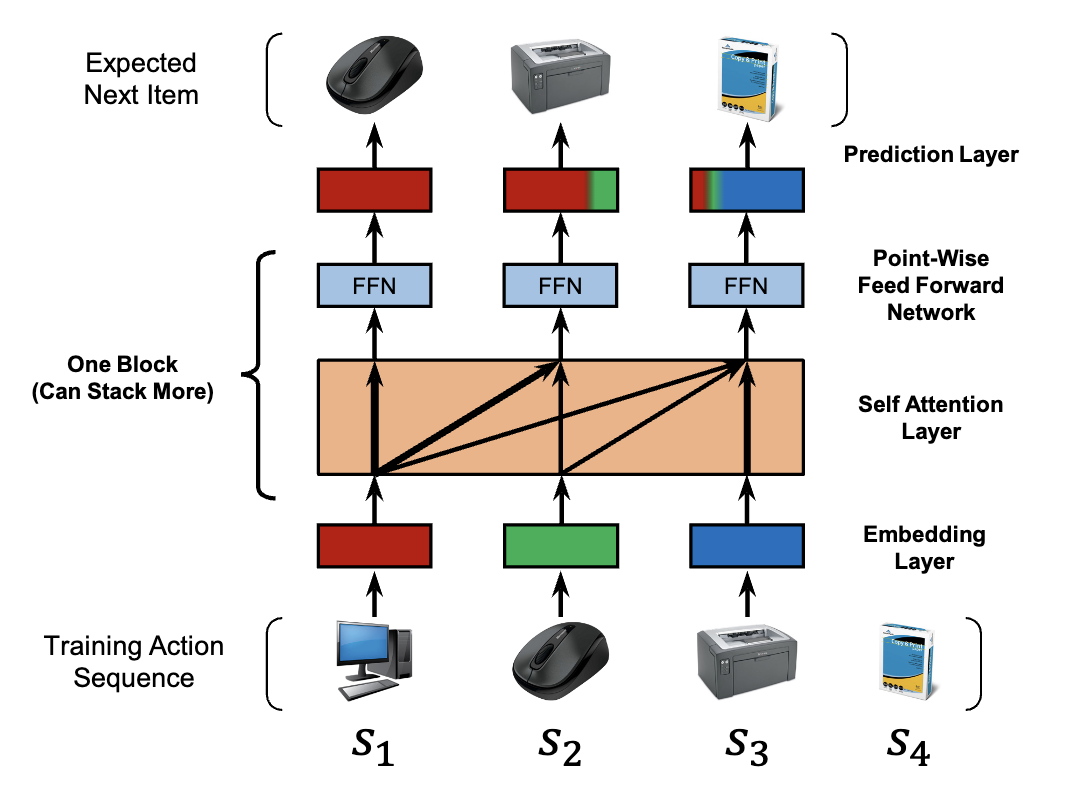
\includegraphics[width=70mm]{images/SASRec.png}
}

\frame{
\frametitle{Графовые нейронные сети}
\begin{columns}[onlytextwidth,T]
  \column{\dimexpr\linewidth-43mm-5mm}
  \begin{enumerate}
    \item Итеративная агрегация признаковых представлений соседей (распространение сообщений):
    $$
    n^{(l)}_v = Aggregator_l(\{h^l_u, \forall u \in \mathcal{N}_v\}),$$$$Update: h^{(l + 1)}_v = Updater_l(h_v^{(l)}, n_v^{(l)}).
    $$
    \item Общий способ представление данных в рек. системе, явная утилизация связей высокого порядка (profit), semi-sup.
  \end{enumerate}

  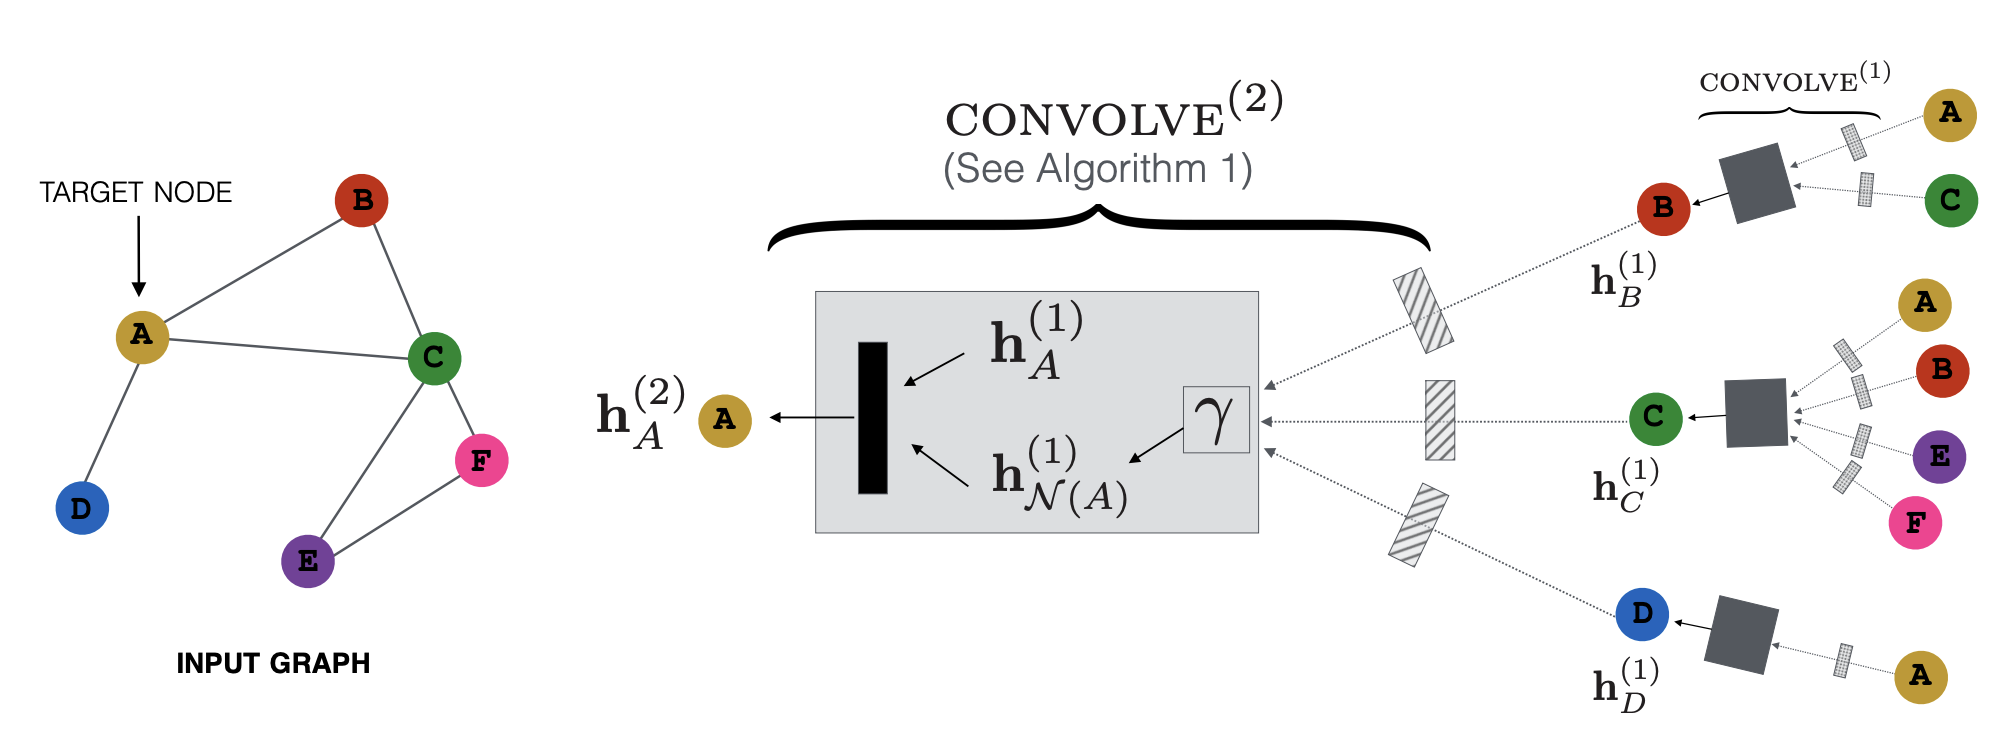
\includegraphics[width=70mm]{images/PinSage.png}
  \column{150mm}
  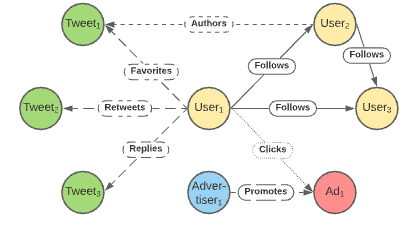
\includegraphics[width=50mm]{images/heter_graph.png}
\end{columns}
}

\frame{
\frametitle{GraphSASRec}
\begin{enumerate}
    \item SASRec - графовая агрегация со стороны пользователя.
    \item Замороженные графовые векторы из GraphSAGE + MLP.
    \item Учет связей второго порядка без доп. накладных расходов.
\end{enumerate}
\hfill
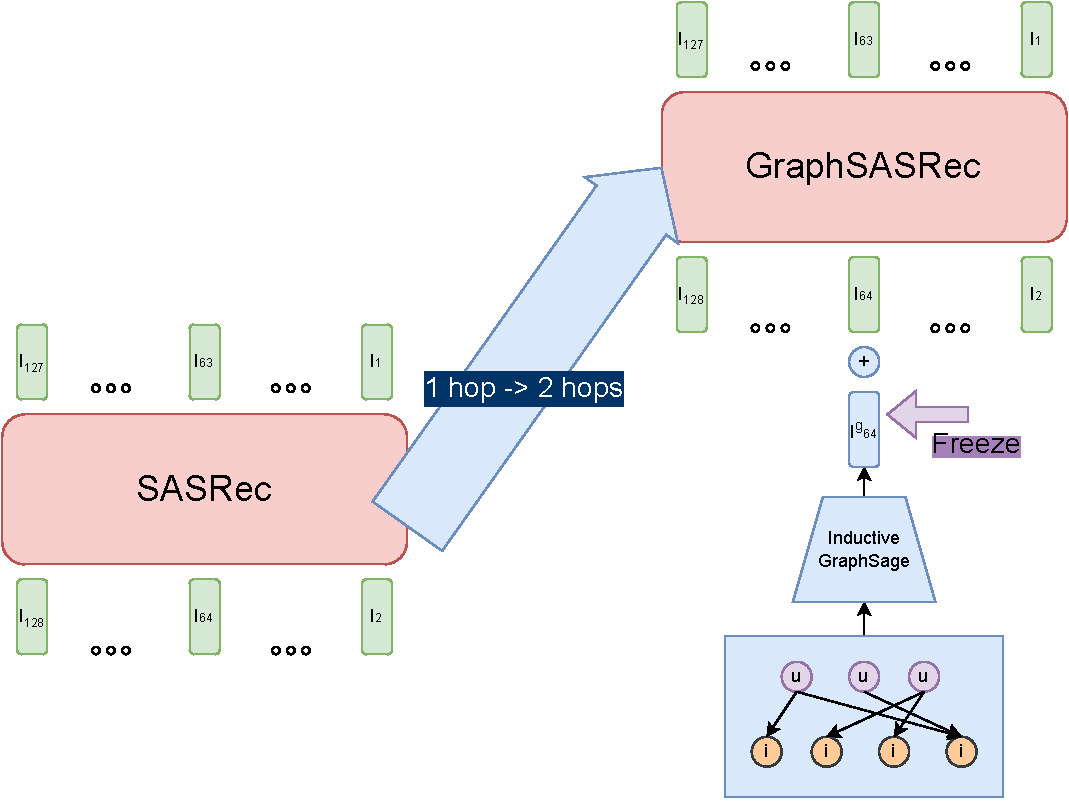
\includegraphics[width=70mm]{images/grpahsasrec2.pdf}
}

\frame{
\frametitle{Корректировка смещения, вызванного семплированием}
\begin{enumerate}
    \item Классическая link-prediction:
    $$
    \mathcal{L}(u, v) = -\log(\sigma(z_u^T z_v)) - \frac{1}{|I_u|} \sum_{v_n \in I} \log(1 - \sigma(z_u^T z_{v_n})),
    $$
    \item В силу разреженности графов:
    $$
    \approx -\log(\sigma(z_u^T z_v)) - \mathbb{E}_{v_n \sim Unif[1, \dots, |I|]} \log(1 - \sigma(z_u^T z_{v_n}))
    $$
    \item In-batch негативы:
    $$
    \approx -\log(\sigma(z_u^T z_v)) - \frac{1}{batch\_size} \sum_{v_n \in Batch} \log(1 - \sigma(z_u^T z_{v_n})).
    $$
    \item (Утв.) Importance-sampling + Монте-Карло:
    $$
    \approx -\log(\sigma(z_u^T z_v)) - \frac{1}{batch\_size} \sum_{v_n \in Batch} \log(1 - \sigma(z_u^T z_{v_n})) \frac{1}{|I| p(v_n)}.
    $$
\end{enumerate}
}

\frame{
\begin{enumerate}
    \item NDCG@10: +22\%
\end{enumerate}

\hfill

\includegraphics[width=70mm]{images/table1.png}
\hfill
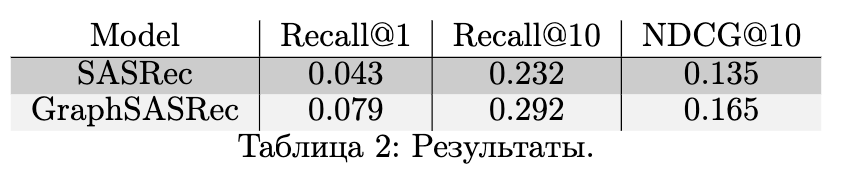
\includegraphics[width=70mm]{images/table2.png}
}

\frame{
\frametitle{Выводы}
\begin{enumerate}
    \item Учет связей второго порядка привел к улучшению качества.
    \item Дальнейшие улучшения: рассмотрение более гетерогенных графов, усложнение графовых архитектур и учет связей высших порядков.
\end{enumerate}
}

% \frame{
% \frametitle{GNN: текущая попытка}
% \begin{columns}[onlytextwidth,T]
%   \column{\dimexpr\linewidth-43mm-5mm}
%   \begin{enumerate}
%     \item $p(interaction|user, item, type)$ / $p(item|user, type)$. 
%     \item Обучаемые айдишники.
%     \item Loss: BCE или Symmetric fps (важно!)
%     \item 2 типа вершин: user, item.
%     \item 4 типа ребер (без них хуже).
%   \end{enumerate}

%   \includegraphics[width=50mm]{images/fps3.png}
  
%   \column{150mm}

%   \includegraphics[width=40mm]{images/now1.pdf}
% \end{columns}
% }

\end{document}